\documentclass[11pt,letterpaper]{article}
\usepackage[utf8]{inputenc}
\usepackage[utf8]{vietnam}
\usepackage{naaclhlt2016}
\usepackage{times}
\usepackage{url}
\usepackage{latexsym}
\usepackage{multirow}
\usepackage{amssymb}
\usepackage{amsthm}
\usepackage{color}
\usepackage{latexsym}
\setlength\titlebox{4cm}

\usepackage{amsmath}
\usepackage{verbatim}
\usepackage{tikz-qtree}
\usepackage{tikz}
\usetikzlibrary{shapes.geometric}
\usetikzlibrary{shapes.arrows}
\usetikzlibrary{patterns}
\usetikzlibrary{chains}
\usetikzlibrary{calc}

\naaclfinalcopy
\def\naaclpaperid{521}

\newtheorem{conjecture}{Conjecture}
\newcommand{\feature}[1]{\ensuremath{\texttt{#1}}}
\newcommand{\pf}[1]{\ensuremath{\textsl{#1}}}
\newcommand{\catstring}[2]{\ensuremath{\pf{#1}\mathbin{:}\feature{#2}}}
\newcommand{\tuple}[2][{}]{\ensuremath{\langle #2 \rangle_{#1}}}
\newcommand{\setcomp}[2]{\ensuremath{\{ #1 \mathrel{|} #2 \}}}
\newcommand{\grammaticalop}[1]{\ensuremath{\textsc{#1}}}
\newcommand{\lexical}{\ensuremath{1}}
\newcommand{\nonlexical}{\ensuremath{0}}

\newcommand{\mcfgrhs}[0]{\ensuremath{\delta}}
\newcommand{\mcfglhs}[0]{\ensuremath{N}}
\newcommand{\mcfgrule}[0]{\ensuremath{N \Rightarrow \mcfgrhs}}

\newcommand{\ensuretext}[1]{#1}
\newcommand{\ignore}[1]{}
\newcommand{\mycomment}[3]{\ensuretext{\textcolor{#3}{[#1 #2]}}}
\newcommand{\cjdmarker}{\ensuretext{\textcolor{blue}{\ensuremath{^{\textsc{C}}_{\textsc{D}}}}}}
\newcommand{\cjd}[1]{\mycomment{\cjdmarker}{#1}{blue}}
\newcommand{\nascomment}[1]{\textcolor{blue}{\textbf{[#1 --\textsc{nas}]}}}
\newcommand{\miguelcomment}[1]{\ignore{\textcolor{red}{\textbf{[#1 --\textsc{MB}]}}}}
\newcommand{\guillaumecomment}[1]{\ignore{\textcolor{orange}{\textbf{[#1 --\textsc{GL}]}}}}

\newcommand{\glmarker}{\ensuretext{\textcolor{orange}{\ensuremath{^{\textsc{G}}_{\textsc{L}}}}}}
\newcommand{\gl}[1]{\mycomment{\glmarker}{#1}{orange}}

\newcommand{\akmarker}{\ensuretext{\textcolor{orange}{\ensuremath{^{\textsc{A}}_{\textsc{K}}}}}}
\newcommand{\ak}[1]{\mycomment{\akmarker}{#1}{orange}}

\newcommand{\ssep}{\,\mid\,}

\newcommand{\thmarker}{\ensuretext{\textcolor{red}{\ensuremath{^{\textsc{T}}_{\textsc{H}}}}}}
\newcommand{\thcomment}[1]{\mycomment{\thmarker}{#1}{red}}
\newenvironment{itemizesquish}{\begin{list}{\setcounter{enumi}{0}\labelitemi}{\setlength{\itemsep}{-0.25em}\setlength{\labelwidth}{0.5em}\setlength{\leftmargin}{\labelwidth}\addtolength{\leftmargin}{\labelsep}}}{\end{list}}

\DeclareMathOperator{\logadd}{logadd}
\DeclareMathOperator*{\argmax}{\arg\!\max}


\title{Các kiến trúc Nơ-ron trong Nhận dạng Thực thể định danh
\Thanks{Bản dịch của bài báo khoa học 
\textbf{Neural Architectures for Named Entity Recognition}
\textit{(https://arxiv.org/abs/1603.01360)} 
thực hiện bởi Phạm Hữu Danh, sinh viên lớp KTPM2014, khoa Công nghệ Phần mềm,
trường Đại học Công nghệ thông tin, Đại học Quốc gia Thành phố Hồ Chí Minh.}}

\author{Guillaume Lample$^{\spadesuit}$ ~ Miguel Ballesteros$^{\clubsuit\spadesuit}$ \\ 
  \textbf{Sandeep Subramanian$^{\spadesuit}$ ~ Kazuya Kawakami$^\spadesuit$ ~ Chris Dyer$^{\spadesuit}$}\\
  $^\spadesuit$Carnegie Mellon University ~~ $^\clubsuit$NLP Group, Pompeu Fabra University \\
  {\tt $\{$glample,sandeeps,kkawakam,cdyer\}@cs.cmu.edu,} \\
  { \tt miguel.ballesteros@upf.edu}}
\date{}

\begin{document}

\maketitle

\begin{abstract}
Các hệ thống \textit{Nhận dạng thực thể định danh} tiên tiến nhất hiện nay phụ thuộc nhiều vào các feature thủ công và kiến thức theo từng lĩnh vực, để học một cách hiệu quả từ ngữ liệu huấn luyện có giám sát \textit{(supervised training corpor)} nhỏ, có sẵn. 
Trong bài báo này, chúng tôi giới thiệu hai Kiến trúc Nơ-ron mới - một kiến trúc dựa trên LSTM hai chiều cùng các field ngẫu nhiên có điều kiện, kiến trúc còn lại xây dựng và phân đoạn nhãn bằng cách sử dụng một cách tiếp cận dựa trên transition mà chúng tôi lấy cảm hứng từ những shift-reduce parser. 
Những mô hình của chúng tôi dựa trên hai nguồn dữ liệu về từ vựng: những word representation dựa-trên-kí-tự được học từ ngữ liệu có giám sát và những word representations không-có-giám-sát \textit{(unsupervised)} được học từ ngữ liệu không có chú thích.
Những mô hình của chúng tôi có được hiệu suất tiên tiến nhất mà không phải dùng đến bất kỳ kiến thức cụ thể về ngôn ngữ hoặc resource như gazetteer.\footnote{Mã nguồn của hai hệ thống NER LSTM-CRF và Stack-LSTM được cung cấp tại: \url{https://github.com/glample/tagger} và \url{https://github.com/clab/stack-lstm-ner}}
\end{abstract}

\section{Giới thiệu}
\textit{Nhận dạng thực thể định danh (Named Entity Recognition - NER)} là vấn đề thách thức trong lĩnh vực học máy. 
Một mặt, trong hầu hết các ngôn ngữ và lĩnh vực, chỉ có một số lượng nhỏ các tập dữ liệu huấn luyện có giám sát. 
Mặt khác, có rất ít những quy ước \textit{(constraint)} đối với các loại từ để có thể là tên riêng, vì vậy việc tổng quát hoá từ tập dữ liệu mẫu nhỏ trở nên rất khó khăn.
Do đó, các feature chính tả được xây dựng cẩn thận và các resource kiến thức cụ thể về ngôn ngữ, như gazetteer, được sử dụng rộng rãi để giải quyết vấn đề này. 
Thật không may, các resource và feature cụ thể của ngôn ngữ rất tốn kém khi phát triển các ngôn ngữ mới và lĩnh mới, trở thành một thách thức cho việc thích nghi của NER. 
\textit{Học không có giám sát (unsupervised learning)} từ các ngữ liệu không có chú thích trở thành một phương án thay thế để có thể khái quát hóa tốt hơn từ một lượng nhỏ giám sát. 
Tuy nhiên, ngay cả các hệ thống đã dựa nhiều vào các feature không có giám sát~\cite[\emph{inter alia}]{collobert2011natural,turian:2010,lin2009phrase,ando:2005} đã sử dụng chúng để hỗ trợ tăng thêm, thay vì thay thế, các feature thủ công (ví dụ: kiến thức về chữ viết hoa và các loại kí tự trong một ngôn ngữ cụ thể) và các kiến thức chuyên ngành (ví dụ: gazetteer).

Trong bài báo này, chúng tôi giới thiệu các kiến trúc nơ-ron cho NER mà không sử dụng tài nguyên cụ thể của ngôn ngữ hoặc các feature vượt quá số lượng nhỏ dữ liệu huấn luyện có giám sát và các tập dữ liệu không có nhãn. 
Những mô hình của chúng tôi được thiết kế để bắt hai intuition \textit{ (khả năng hiểu ngay lập tức)}. 
Đầu tiên, vì tên riêng thường bao gồm nhiều token, lý luận hợp lí để tagging mỗi token là rất quan trọng. 
Ở đây chúng tôi so sánh hai mô hình, (i)~LSTM hai chiều với một lớp ngẫu nhiên có điều kiện tuần tự nằm trên nó~(LSTM-CRF; \S\ref{lstmcrf}), và (ii)~một mô hình mới xây dựng và phân đoạn nhãn của các câu đầu vào bằng cách sử dụng một thuật toán lấy cảm hứng từ transition-based parsing với các state được tái thể hiện bởi stack LSTMS~(S-LSTM; \S\ref{stacklstm}). 
Thứ hai, những evidence mức token ``để xác định tên riêng'' bao gồm những orthographic evidence (Từ được gắn thẻ là tên riêng trông như thế nào?) và distributional evidence (Những từ được gắn thẻ là tên riêng thường xảy ra ở đâu trong ngữ liệu?). 
Để lấy được orthographic sensitivity, chúng tôi sử dụng mô hình word representation dựa-trên-kí-tự~\cite{ling:2015}, để lấy được distributional sensitivity, chúng tôi kết hợp các word representation này với distributional representations~\cite{mikolov2013distributed}.
Word representation của chúng tôi kết hợp cả hai, và tỉ lệ dropout training được sử dụng để giúp các mô hình học cách tin tưởng cả hai nguồn evidence~(\S\ref{sec:words}).

Các thử nghiệm trong tiếng Anh, Hà Lan, Đức và Tây Ban Nha cho thấy chúng tôi có thể đạt được hiệu suất NER tiến tiến nhất với mô hình LSTM-CRF ở Hà Lan, Đức và Tây Ban Nha và rất gần với mức tiên tiến nhất trong tiếng Anh mà không có bất kỳ feature thủ công hoặc gazetteer. 
Thuật toán dựa trên transition cũng vượt qua các kết quả tốt nhất được xuất bản trước đó trong nhiều ngôn ngữ, mặc dù hiệu quả của nó kém hơn so với mô hình LSTM-CRF.

\section{Mô hình LSTM-CRF}
\label{lstmcrf}
Chúng tôi cung cấp một mô tả ngắn gọn về LSTM và CRF, và trình bày kiến trúc hybrid tagging. Kiến trúc này tương tự cái đã được trình bày bởi \newcite{collobert2011natural} và \newcite{huang:2015}.

\subsection{LSTM}
\label{sec:lstm}

Những mạng Nơ-ron Hồi quy (Recurrent neural networks - RNNs) là tập hợp các mạng Nơ-ron mà hoạt động trên dữ liệu tuần tự \textit{(sequential data)}.
Chúng nhận đầu vào là một chuỗi các vec-tơ $(\mathbf{x}_1, \mathbf{x}_2, \ldots, \mathbf{x}_n)$ và trả về một chuỗi khác $(\mathbf{h}_1, \mathbf{h}_2, \ldots, \mathbf{h}_n)$ tái thể hiện cho các thông tin về chuỗi của mỗi bước đầu vào.
Mặc dù RNNs trên lý thuyết có thể họ những dependency dài, nhưng trên thực tế chúng thất bại khi làm thế và có xu hướng trở trên thiên vị \textit{(biased toward)} với những đầu vào gần nhất trong chuỗi \cite{bengio1994learning}. 
Mạng bộ nhớ dài hạn-ngắn hạn \textit{(Long Short-term Memory Networks - LSTMs)} đã được thiết để khắc phục vấn đề này bằng cách kết hợp một cell bộ nhớ và đã được chứng minh là nắm bắt được các dependency trong một khoảng dài. 
Nó làm vậy bằng cách sử dụng một số cổng kiểm soát tỷ lệ đầu vào cung cấp cho các cell nhớ, và tỷ lệ từ cổng phía trước để quên~\cite{hochreiter:1997}.
Chúng tôi sử dụng cách implement sau:
\\
\begin{align*}
\mathbf{i}_{t} &= \sigma(\mathbf{W}_{xi}\mathbf{x}_{t} + \mathbf{W}_{hi}\mathbf{h}_{t-1} + \mathbf{W}_{ci}\mathbf{c}_{t-1} + \mathbf{b}_{i})\\
% \mathbf{f}_{t} &= \sigma(\mathbf{W}_{xf}\mathbf{x}_{t} + \mathbf{W}_{hf}\mathbf{h}_{t-1}+\mathbf{W}_{cf}\mathbf{c}_{t-1} + \mathbf{b}_{f})\\
\mathbf{c}_{t} &= (1 - \mathbf{i}_{t})\odot\mathbf{c}_{t-1} +\\
&\qquad \mathbf{i}_{t}\odot \tanh(\mathbf{W}_{xc}\mathbf{x}_{t} + \mathbf{W}_{hc}\mathbf{h}_{t-1} + \mathbf{b}_{c})\\
\mathbf{o}_{t} &= \sigma(\mathbf{W}_{xo}\mathbf{x}_{t} + \mathbf{W}_{ho}\mathbf{h}_{t-1} + \mathbf{W}_{co}\mathbf{c}_{t} + \mathbf{b}_{o})\\
\mathbf{h}_{t} &= \mathbf{o}_{t}\odot\tanh(\mathbf{c}_{t}),
\end{align*}
với $\sigma$ làm một hàm element-wise sigmoid, và $\odot$ là element-wise product.

Với một câu cho trước $(\mathbf{x}_1, \mathbf{x}_2, \ldots, \mathbf{x}_n)$ bao gồm $n$ từ, mỗi từ được tái thể hiện bằng một vec-tơ $d$-chiều, một LSTM sẽ tính một tái thể hiện $\overrightarrow{\mathbf{h}_t}$ ngữ cảnh bên trái \textit{(left context representation)} của mỗi từ $t$ trong câu. 
Tất nhiên, cũng sẽ xuất ra một tái thể hiện ngữ cảnh bên phải $\overleftarrow{\mathbf{h}_t}$ \textit{(right context representation)} để có thêm các thông tin hữu ích. 
Điều này có thể đạt được bằng một LSTM thứ hai được sử dụng để đọc cùng một câu theo hướng ngược lại. 
Chúng tôi xem cái đầu tiên là \textit{forward LSTM} và cái phía sau là \textit{backward LSTM}. 
Đây là hai mạng riêng biệt với các thông số khác nhau. 
Một cặp forward và backward LSTM được gọi là LSTM hai chiều~\cite{graves:2005}.

Word representation của một từ được sử dụng trong model này được lấy từ việc nối lại tái thể hiện ngữ cảnh bên trái và bên phải của nó, $\mathbf{h}_{t} = [\overrightarrow{\mathbf{h}_{t}} ; \overleftarrow{\mathbf{h}_{t}}]$. Những thuộc tính này tái hiện một cách hiệu quả từ trong ngữ cảnh, giúp ích cho nhiều ứng dụng gắn nhãn.

\subsection{Những mô hình gắn nhãn CRF}
\label{sec:crf}
Một mô hình gắn nhãn rất đơn giản---nhưng cực kỳ hiệu quả--- là sử dụng $\mathbf{h}_t$ như một tính feature để ra những quyết định gắn nhãn một cách độc lập cho mỗi đầu ra $y_t$~\cite{ling:2015}. 
Mặc dù mô hình này thành công trong các vấn đề đơn giản như POS tagging, nhưng các quyết định phân loại độc lập của nó đang hạn chế khi có sự phụ thuộc mạnh mẽ giữa các nhãn đầu ra. 
NER là một việc tương tự, bởi vì ``ngữ pháp'' sẽ đặc trưng cho trình tự giải nghĩa của các tag áp đặt một số quy ước cứng  (ví dụ: I-PER không thể theo sau B-LOC; xem \S\ref{IOBES} để biết thêm chi tiết) dẫn đến việc không thể nào ứng dụng mô hình với các giả định độc lập.

Do đó, thay vì lập ra mô hình quyết định gắn nhãn độc lập, chúng tôi mô hình chúng kết hợp với nhau sử dụng các field ngẫu nhiên có điều kiện~\cite{lafferty2001conditional}.

Với một câu đầu vào
$$\mathbf{X} = (\mathbf{x}_1, \mathbf{x}_2, \ldots, \mathbf{x}_n),$$
Chúng tôi xem xét $\mathbf{P}$ là một ma trận điểm ở đầu ra bởi một mạng LSTM hai chiều. $\mathbf{P}$ có kích thước $n~\times~k$, với $k$ là số lượng tag riêng biệt, và $P_{i, j}$ ứng với score của tag thứ $j^{th}$ của từ thứ $i^{th}$ trong câu. Đối với một chuỗi các dự đoán
$$\mathbf{y} = (y_1, y_2, \ldots, y_n),$$
Chúng tôi định nghĩa score của nó là
$$s(\mathbf{X}, \mathbf{y})=\sum_{i=0}^{n} A_{y_i, y_{i+1}} + \sum_{i=1}^{n} P_{i, y_i}$$
với $\mathbf{A}$ là ma trận của transition scores, trong đó $A_{i, j}$ là score của transition từ tag $i$ đến tag $j$. $y_0$ và $y_n$ là những tag \textit{bắt đầu} và \textit{kết thúc} của một câu, mà chúng tôi thêm vào tập hợp cái tag có khả năng. 
Do đó $\mathbf{A}$ là một ma trận vuông với kích thước $k+2$.
\\
\\
Một softmax trên tất cả tag có khả năng cho ra một xác suất cho trình tự $\mathbf{y}$:
$$p(\mathbf{y} | \mathbf{X}) = \frac{
	e^{s(\mathbf{X}, \mathbf{y})}
}{
	\sum_{\mathbf{\widetilde{y}} \in \mathbf{Y_X}} e^{s(\mathbf{X}, \mathbf{\widetilde{y}})}
}.$$
Trong quá trình train, chúng tôi tối đa \textit{log-probability} của các sequence tag đúng:
\\
\begin{align}
\log(p(\mathbf{y} | \mathbf{X})) &= s(\mathbf{X}, \mathbf{y}) - \log \left( \sum_{\mathbf{\widetilde{y}} \in \mathbf{Y_X}} e^{s(\mathbf{X}, \mathbf{\widetilde{y}})} \right) \nonumber \\
&= s(\mathbf{X}, \mathbf{y}) - \underset{{\mathbf{\widetilde{y}} \in \mathbf{Y_X}}}{\logadd}\ s(\mathbf{X}, \mathbf{\widetilde{y}}), \label{eq:crf}
\end{align}
với $\mathbf{Y_X}$ thể hiện cho tất cả các trình tự tag có khả năng (kể cả những cái không thỏa IOB format) cho một câu $\mathbf{X}$. Từ công thức trên, hiển nhiên rằng chúng tôi khuyến khích mạng nơ-ron của chúng tôi cho ra một trình tự các nhãn đầu ra hợp lệ. 
Khi giải mã, chúng tôi dự đoán trình tự đầu ra đạt được điểm tối đa được đưa ra bởi công thức:
\begin{align}
\mathbf{y}^* = \argmax_{\mathbf{\widetilde{y}} \in \mathbf{Y_X}}{s(\mathbf{X}, \mathbf{\widetilde{y}})}. \label{eq:vit}
\end{align}

Bởi vì chúng tôi chỉ mô hình các bigram interaction giữa các đầy ra, cả quá trình summation ở công thức Eq.~\ref{eq:crf} và maximum trình tự posteriori $\mathbf{y}^*$ ở công thức Eq.~\ref{eq:vit} đều có thể tính bằng cách sử dụng quy hoạch động \textit{(dynamic programming)}.

\begin{figure}
  \centering
    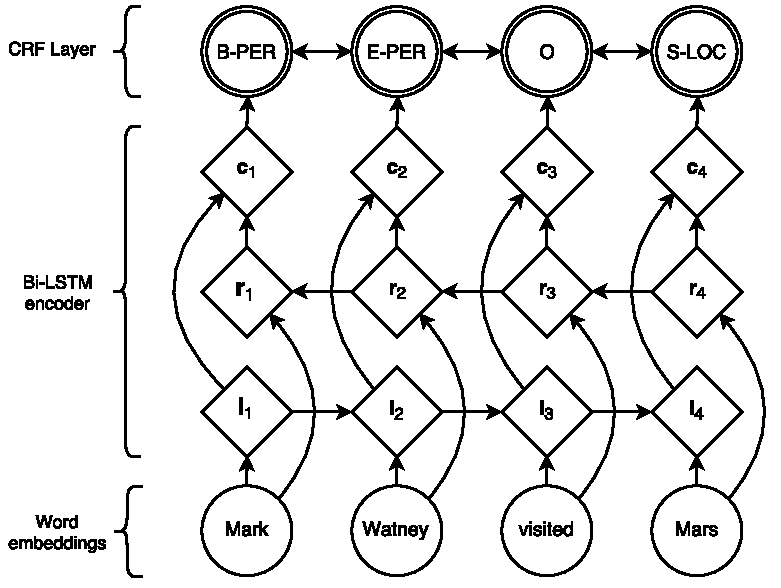
\includegraphics[scale=0.64]{bilstm-crf4}
  \caption{Kiến trúc chính của mạng nơ-ro. Các word embedding được đưa vào LSTM 2 chiều. $\mathbf{l}_i$ thể hiện từ thứ $i$ và ngữ cảnh bên trái của nó, $\mathbf{r}_i$ thể hiện cho từ thứ $i$ và ngữ cảnh bên phải của nó. Việc kết hợp hai vec-tơ sẽ cho ra một representation của từ thứ $i$ trong ngữ cảnh của nó, $\mathbf{c}_i$.}
  \label{fig:bilstm-crf}
\end{figure}

\subsection{Tham số hóa và Training}
Những score của mỗi quyết định gán nhãn cho từng token (các giá trị $P_{i,y}$) được định nghĩa là những kết quả nhân ma trận giữa embedding của một từ trong ngữ cảnh đã được tính với một LSTM hai chiều---chính xác là nó giống như mô hình POS tagging của \newcite{ling:2015} và chúng được kết hợp với các bigram compatibility score (các giá trị $A_{y,y'}$). Kiến trúc này được mô tả ở Hình \ref{fig:bilstm-crf}. 
Vòng tròn đại diện cho các biến được quan sát, kim cương là các chức năng xác định của parent, và vòng tròn đôi là các biến ngẫu nhiên.

Các tham số của mô hình này là các ma trận của những bigram compatibility score $\mathbf{A}$, và 
các tham số phát sinh cho ma trận $\mathbf{P}$, cụ thể là các tham số của LSTM hai chiều, các feature trọng số của đường và word embeddings. Như đã đề cập trong phần~\ref{sec:crf}, có $\mathbf{x}_i$ biểu thị một trình tự của các word embedding chỗ mỗi từ trong câu, và $y_i$ là những tag tương ứng. Chúng tá quay lại thảo luận làm cách nào các embedding $\mathbf{x}_i$ được mô hình hóa trong Phần~\ref{sec:words}. Trình tự của các word embedding được xem như đầu vào cho LSTM hai chiều, sẽ trả về một tái thể hiện ngữ cảnh bên trái và bên phải cho mỗi từ như được giải thích ở ~\ref{sec:lstm}.

Những representation này được kết hợp ($\mathbf{c}_i$) và chiếu tuyến tính lên một layer có kích thước bằng với số lượng các tag riêng biệt. 
Thay vì sử dụng đầu ra softmax cho layer này, chúng tôi sử dụng một CRF, đã được mô tả trước đó, để tính cho các tag lân cận,  cho ra dự đoán cuối cùng cho mỗi từ $y_i$. 
Ngoài ra, chúng tôi quan sát thấy rằng khi thêm vào một hidden layer giữa $\mathbf{c}_i$ và CRF layer đã giải thiện đôi chút kết quả của chúng thôi.

\subsection{Tagging Schemes}
\label{IOBES}

Nhiệm vụ của nhận dạng thực thể định danh là gán đúng những nhãn định danh thực thể vào mỗi từ trong một câu.
Một thự thể định danh đơn lẻ có thể gồm nhiều token trong câu. Các câu thì thường được thể hiện dưới IOB format (Inside, Outside, Beginning), chính là nơi mà những token được gán nãn là B-\textit{label} nếu token là bắt đầu của một thực thế định danh, I-\textit{label} nếu nó nằm trong một thực thể định danh nhưng không phải là cái đầu tiên, O-\textit{label} cho những token còn lại. Tuy nhiên, chúng tôi đã quyết định sử dụng IOBES tagging scheme, một sự mở rộng của IOB, thường được sử dụng cho nhận dạng thực thể định danh, nó mã hóa thông tin về các thực thể singleton (S) và đánh dấu một cách rõ ràng điểm kết thúc của thực thể định danh (E). Sử dụng scheme này, việc đánh dấu một từ là I-\textit{label} với độ confidence cao sẽ thu hẹp lại sự lựa chọn cho các từ trong trình tự là I-\textit{label} hoặc E-\textit{label}, tuy nhiên, IOB scheme chỉ có khả năng xác định rằng từ tiếp theo không thể là bộ phận của một nhãn khác. \newcite{ratinov2009design} và \newcite{dai2015enhancing} đã chứng minh rằng một tagging scheme có khả năng mô tả nhiều hơn sẽ cải thiện hiệu năng của mô hình một chút. Tuy nhiên, chúng tôi không quan sát thấy sự cải thiện có ý nghĩa nào so với IOB tagging scheme.

\section{Mô hình phân đoạn dựa trên transition}
\label{stacklstm}

Là một hướng thay thế cho LSTM-CRF đã được đề cập ở chương trước, chúng tôi phát hiện một kiến trúc mới để phân đoạn và gián nhãn một trình đầu vào sử dụng một thuật toán tương tự như transition-based dependency parsing. Mô hình này xây dựng trực tiếp các representation của tên riêng nhiều token (ví dụ: tên riêng \emph{Mark Watney} được tạo ra vào một representation riêng).

Mô hình này dựa nhiều vào cấu trúc dữ liệu stack để cải thiện việc xây dụng các phân đoạn của đầu vào. Để có được các representation của stack này cho việc dự đoán các action tiếp theo, chúng tôi sử dụng Stack-LSTM được trình bày bởi \newcite{dyer:2015}, trong đây LSTM được tăng cường với một ``stack pointer''. Trong khin những mô hình LSTM tuần tự sẽ đi từ trái sang phải, stack LSTM cho phép embedding của một stack các objects đều được thêm vào (sử dụng push operation) và loại ra (sử dụng pop operation). Điều này cho phép Stack-LSTM làm việc giống như một stack để bảo trì một ``summary embedding'' cho dữ liệu của nó. Chúng tôi gọi mô hình này là Stack-LSTM hoặc S-LSTM model cho đơn giản. 

Cuối cùng, chúng tôi giới thiệu độc giả quan tâm tới bài báo gốc \cite{dyer:2015} để biết chi tiết về mô hình Stack-LSTM vì trong bài báo này, chúng tôi chỉ sử dụng cùng một kiến trúc thông qua một thuật toán chuyển tiếp mới được trình bày trong Phần sau đây.

\subsection{Thuật toán Phân đoạn}

Chúng tôi đã thiết kế một transition inventory được mô tả ở hình~\ref{fig:parser}, cái mà được lấy cảm hứng từ những transition-based parsers, chính xác là arc-standard parser của \newcite{nivre2004}. Trong thuật toán này, chúng tôi sử dụng hai stack (\emph{đầu ra} được chỉ định và \emph{stack} tái thể hiện, tương ứng với, phân đoạn hoàn toàn và không gian scratch) và một \emph{bộ đêm} chưa các chữ chưa được xử lí. Transition inventory sẽ chứa các transition sau: \textsc{shift} transition di chuyển một từ từ bộ đệm đến stack, \textsc{out} transition di chuyển một từ từ bộ đêm đến thẳng stack đầu ra khi \textsc{reduce}$(y)$ transition đẩy toàn bộ items từ phía trên của stack tạo thành một  ``chunk,'' được gán với nhãn $y$, và đẩy một representation của chunk này vào stack đầu ra. Thuận toán hoàn tất khi cả stack và bộ đếm đều rỗng. Thuật toán được mô tả trong Hình \ref{fig:parser}, cho thấy một trình tự các operation cần thiết để xử lí câu \emph{Mark Watney visited Mars}. 

\begin{figure*}
\begin{small}
\centering
\begin{tabular}{lll|l|lll|c}
\textbf{Out}$_t$ & \textbf{Stack}$_t$ & \textbf{Buffer}$_t$ & \textbf{Action} & \textbf{Out}$_{t+1}$ & \textbf{Stack}$_{t+1}$ & \textbf{Buffer}$_{t+1}$ & \textbf{Segments} \\
\hline
$O$ & $S$ & $(\mathbf{u},u),B$ & \textsc{shift} & $O$ & $(\mathbf{u},u),S$ & $B$ & --- \\ %\hline
$O$ & $(\mathbf{u},u),\ldots,(\mathbf{v},v),S$ & $B$  &$\textsc{reduce}(y)$ & $g(\mathbf{u},\ldots,\mathbf{v},\mathbf{r}_y),O$ & $S$ & $B$ & $(u\ldots v,y)$ \\
$O$ & $S$ & $(\mathbf{u},u),B$ & \textsc{out} & $g(\mathbf{u},\mathbf{r}_{\varnothing}),O$ & $S$ & $B$ & ---
\end{tabular}
\end{small}
\caption{Transitions of the Stack-LSTM model indicating the action applied and the resulting state. \guillaumecomment{this first sentence is maybe a little bit confusing} Bold symbols indicate (learned) embeddings of words and relations, script symbols indicate the corresponding words and relations.}
\label{fig:parser}
\end{figure*}

\begin{figure*}[t]
  \begin{center}
    \centering
    \begin{scriptsize}
      \begin{tabular}{lllll}\textbf{Transition}&\textbf{Output}&\textbf{Stack}&\textbf{Buffer}&\textbf{Segment}\\
      \hline
        &[]&[]&[Mark, Watney, visited, Mars]&\\
        \textsc{Shift}&[]&[Mark]&[Watney, visited, Mars]&\\
        \textsc{Shift}&[]&[Mark, Watney]&[visited, Mars]&\\
        \textsc{REDUCE(PER)}&[(Mark Watney)-PER]&[]&[visited, Mars]& (Mark Watney)-PER\\
        \textsc{OUT}&[(Mark Watney)-PER, visited]&[]&[Mars]&\\
        \textsc{SHIFT}&[(Mark Watney)-PER, visited]&[Mars]&[]&\\
        \textsc{REDUCE(LOC)}&[(Mark Watney)-PER, visited, (Mars)-LOC]&[]&[]& (Mars)-LOC\\
      \end{tabular}
    \end{scriptsize}
    \caption{Transition sequence for \emph{Mark Watney visited Mars} with the Stack-LSTM model.}
    \label{parsingexample}
  \end{center}
\end{figure*}

Mô hình này đã được tùy chỉnh tham số để định nghĩa xác suất phân phối các action trong mỗi time step, cho trước nội dung hiện tại của stack, bộ đệm và đầu ra, cũng như lịch sử các action đã thực hiện. Theo như \newcite{dyer:2015}, chúng tôi sử dụng stack LSTM để tính toán một embedding có chiều cố định cho mỗi phần tử, và sau đó kết nối chúng để có state của toàn bộ thuật toán. Representation này được sử dụng để định nghĩa một phân phối trên toàn bộ các action có khả năng mà có thể lấy ra ở mỗi step. Mô hình được train để tối đa hóa xác suất có điều kiện của các trình tự của các reference action (chính xác là từ ngữ liệu huấn luyện đã được đánh nhãn) cho các câu đầu vào. Để đánh nhãn một câu đầu vào mới ở thời điểm test, action có khả năng lớn nhất sẽ được chọn một cách tham lam cho tới khi thuật toán chạm state kết thúc. Mặc dù điều này không đảm bảo rằng sẽ tìm được sự tối ưu toàn bộ nhưng nó hiệu quả trong thực tế, Bởi vì mỗi token được di chuyển trực tiếp đến đầu ra (1 action) hoặc đến stack rồi đến đầu ra (2 action), tổng số lượng action cần cho một câu có độ dài $n$ tối đa là $2n$.

Cần lưu ý rằng bản chất của mô hình thuật toán này làm cho nó không đồng nhất với tagging scheme được sử dụng vì nó trực tiếp dự đoán các chunk nhãn.

\subsection{Representing Labeled Chunks}

Khi $\textsc{reduce}(y)$ operation được thực thi, thuật toán shift một trình tự các token (cùng với các vec-tơ embedding của chúng) từ stack đến buffer đầu ra như một chunk đơn hoàn tất. Để tính một embedding của chuỗi này, chúng tôi chạy một LSTM hai chiều trên những embedding của các tokens thành phần cùng với một token đại diện cho loại của chunk đang xác định $y$. Hàm này được cho như $g(\mathbf{u}, \ldots, \mathbf{v},\mathbf{r}_y)$ với $\mathbf{r}_y$ là một learned embedding của loại nhãn. Do đó, bộ đệm đầu ra chứa các vec-tơ representation đơn cho mỗi chunk nhãn được tạo ra, thay vì chiều dài của nó.

\section{Word Embeddings đầu vào}\label{sec:words}
Những layer đầu vào cho cả hai mô hình của chúng tôi đều là những vec-tơ representation của những từ đơn. Việc học từ những representation độc lập cho các loại từ lấy từ một tập dữ liệu huấn luyện NER có giới hạn là một vấn đề khó khăn: có rất nhiều thông số để ước tính một cách đáng tin cậy. Bởi vì nhiều ngôn ngữ có orthographic hoặc morphological evidence để một thứ gì đó là tên riêng (hoặc không là tên riêng), chúng tôi muốn những representation mà có thể sensitive với các phát âm của từ. Do đó chúng tôi sử dụng mô hình xây dựng representation của word từ những representation của kí tự mà chúng được hợp thành~(\ref{sec:character-model}).
Intuition thứ hai của chúng tôi là những tên riêng, thường khá đa dạng một cách riêng lẻ, xuất hiện trong các ngữ cảnh thông thường trong ngữ liệu lớn. Do đó chúng tôi dùng những embedding học từ một ngữ liệu lớn, sensitive với thứ tự sắp xếp của từ~(\ref{sec:pretrained}). Cuối cùng, để ngăn ngừa những mô hình dựa vào một representation quá nhiều, chúng tôi dùng dropout training và nhận thấy điều này rất quan trọng cho hiệu suất tổng quát~(\ref{sec:dropout}).

\subsection{Mô hình dựa trên kí tự của từ}
\label{sec:character-model}


\begin{figure}
  \centering
    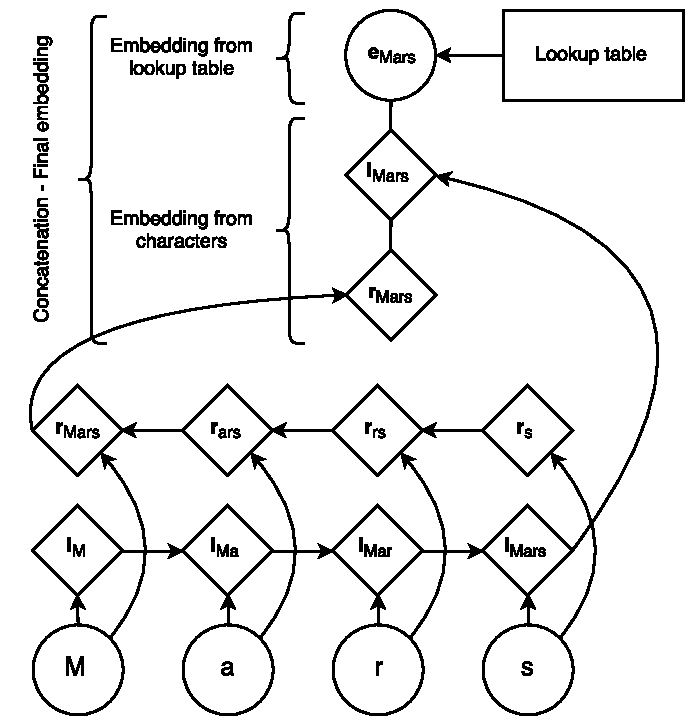
\includegraphics[scale=0.68]{char-model4}
  \caption{Những embedding kí tự của từ ``Mars'' được cho vào một LSTM hai chiều. Chúng tôi kết hợp những đầu ra cuối cùng với một embedding lấy ra từ lookup table để có được một representation cho từ này.}
  \label{fig:char-model}
\end{figure}

Một sự khác biệt quan trọng trong cách làm của chúng tôi với những hướng tiếp cạnh trước là chúng tôi học các feature ở mức kí tự khi training thay vì cài đặt thủ công các thông tin tiền tố và hậu tố về từ. hojc từ embedding mức kí tự có lợi thế trong việc học representation cụ thể cho công việc và lĩnh vực hiện tại. Chúng đã được chứng minh là hữu ích cho những ngôn ngữ đa hình thái và để xử các vấn đề nằm ngoài từ vựng cho các tác vụ như part-of-speech tagging và mô hình hóa ngôn ngữ \cite{ling:2015} hoặc dependency parsing \cite{lstmemnlp15}.

Hình~\ref{fig:char-model} mô tả kiến trúc của chúng tôi để tạo ra một word embedding của một từ qua những kí tự của nó. Một lookup table kí tự được tạo ra ngẫu nhiên bao gồm một embedding cho mỗi kí tự. Các embedding kí tự tương ứng với mỗi kí tự trong một từ được cung cấp theo hướng trực tiếp và lật ngược cho một forward và một backward LSTM. Embedding cho một từ có nguồn gốc từ kí tự của nó là sự kết hợp của forward và backward representation từ LSTM hai chiều. Representation mức kí tự này sau đó được kết hợp với representation mức từ vựng từ lookup table. Trong quá trình test, từ không có embedding trong lookup table sẽ được map đến UNK embedding. Để train một UNK embedding, chúng tôi thay thế những singletons bằng UNK embedding với xác suất $0.5$. Trong tất cả các thí nghiệm của chúng tôi, hidden dimension của forward và backward LSTM kí tự là $25$ cho mỗi cái, kết quả trong những word representation dựa trên kí tự của chúng tôi có dimension là $50$. 

Các mô hình lặp lại như RNN và LSTM có khả năng mã hóa các chuỗi rất dài, tuy nhiên, chúng có các representation cho xu hướng thiên vị về các đầu vào gần nhất. Với kết quả, chúng tôi mong muốn representation cuối cùng của forward LSTM sẽ là một representation chính xác cho tiền tố của từ, và trạng thái cuối cùng của backward LSTM là một representation tốt hơn  so với tiền tố của nó. Những phương pháp tiếp cận thay thế---đáng chú ý nhất là các mạng xoắn---đã được đề xuất để học representation của từ thông qua kí tự của chúng \cite{zhang2015character,DBLP:journals/corr/KimJSR15}. Tuy nhiên, convnets được thiết kế để khám phá các feature bất biến vị trí của đầu vào. Mặc dù điều này phù hợp với nhiều vấn đề, ví dụ như nhận diện hình ảnh (một con mèo có thể xuất hiện ở bất cứ nơi nào trong bức tranh), chúng tôi cho rằng thông tin quan trọng là phụ thuộc vào vị trí (ví dụ, tiền tố và hậu tố mã hóa thông tin khác với đoạn giữa), làm LSTMs trở thành \emph{a priori} lớp chức năng tốt hơn để mô hình hóa mối quan hệ giữa các từ và các ký tự của chúng.

\subsection{Pretrained embeddings}\label{sec:pretrained}

Theo như \newcite{collobert2011natural}, chúng tôi sử dụng pretrained word embeddings được train trước để khởi tạo lookup table. Chúng tôi quan sát thấy những cải tiến đáng kể bằng cách sử dụng các pretrained word embeddings thay vì những cái được khởi tạo ngẫu nhiên. Embeddings được train trước sử dụng skip-n-gram \cite{skipngram}, một biến thể của word2vec \cite{mikolov2013efficient} chỉ định các vị trí của từ. Những embedding này được tinh chỉnh trong quá trình training.

Word embeddings cho tiếng Tây Ban Nha, Hà Lan, Đức và Anh được train tương ứng bằng dữ liệu Spanish Gigaword version~3, tập ngữ liệu Leipzig, dữ liệu train monolingual tiếng Đức từ 2010 Machine Translation Workshop và English Gigaword version~4 (với những phần của LA Times và NY Times đã được gỡ bỏ).\footnote{\cite{graff2011spanish,biemann2007leipzig,callison2010findings,englishgigaword}}

Chúng tôi sử dụng embedding dimension $100$ cho Tiếng Anh, $64$ cho các ngôn ngữ khác, tần số từ cutoff thấp nhất là $4$, và kích thước cửa số là $8$.

\subsection{Dropout training}\label{sec:dropout}

Những thử nghiệm ban đầu cho thấy những embedding mức kí tự không cải thiện hiệu năng chung khi được sử dụng kết hợp với các pretrained word representation. Để thúc đẩy mô hình phụ thuộc vào tất cả representation, chúng tôi dùng dropout training \cite{dropout}, ứng dụng một dropout mask ở embedding layer cuối cùng trước khi cho đầu vào đến LSTM hai chiều như trong Hình \ref{fig:bilstm-crf}. Chúng tôi quan sát thấy sự cải tiến đáng kể về hiệu năng trong mô hình sau khi sử dụng dropout (xem bảng~\ref{results-diff-config}).

\section{Các thí nghiệm}\label{sec:experiments}

Phần này trình bày các phương pháp chúng tôi sử dụng để đào tạo các mô hình của chúng tôi, kết quả thu được từ các task khác nhau và sự tác động của việc cấu hình mạng đối với hiệu suất của mô hình.

\subsection{Training}

Với các mô hình đã giới thiệu, chúng tôi huấn luyện các mạng bằng thuật toán back-propagation cập nhật các tham số của chúng tôi trên mỗi training example, ở từng thời điểm, sử dụng stochastic gradient descent (SGD) với learning rate là $0.01$ và gradient clipping là $5.0$. Nhiều phương pháp đã được giới thiệu để cải thiện hiệu năng của SGD như là Adadelta \cite{adadelta} hoặc Adam \cite{adam}. Mặc dù chúng tôi quan sát convergence sự hội tụ nhanh hơn khi sử dụng những phương pháp ấy, nhưng không có cái này trong chúng có hiệu năng tốt như SGD với gradient clipping.

Mô hình LSTM-CRF của chúng tôi sử dụng một layer đơn cho forward và backward LSTM với dimension được dùng là $10$. Thay đổi số dimension này đã không ảnh hướng nhiều đến hiệu năng của mô hình. Chúng tôi sử dụng tỉ lệ dropout $0.5$. Sử dụng tỷ lệ cao hơn tác động tiêu cực đến kết quả của chúng tôi, trong khi tỷ lệ nhỏ hơn dẫn đến thời gian đào tạo dài hơn.

Mô hình stack-LSTM sử dụng hai layer với mỗi dimension là $100$ cho mỗi stack. Embedding của các actions đã sử dụng composition function có $16$ dimension cho mỗi cái, và embedding đầu ra có dimension $20$. Chúng tôi đã thí nghiệm với những tỉ lệ dropout khác nhau và báo cáo những score sử dụng tỉ lệ dropout tốt nhất cho mỗi ngôn ngữ.\footnote{English (D=$0.2$), German, Spanish and Dutch (D=$0.3$)} Đây là một mô hình tham lam mà áp dụng các hành động tối ưu local cho tới khi cả câu được xử lý, những cải tiến sau này có thể đạt được với beam search \cite{zhang:2011} hoặc training with exploration \cite{ballesteros-arxiv16}.

\subsection{Các tập dữ liệu}

Chúng tôi thử nghiệm mô hình của mình trên nhiều tập dữ liệu khác nhau cho việc nhận dạng thực thể định danh. Để chứng minh khả năng tổng quát của mô hình đối với các ngôn ngữ khác nhau, chúng tôi trình bày các kết quả trên tập dữ liệu CoNLL-2002 và CoNLL-2003 \cite{TjongKimSang:2002:ICS:1118853.1118877,TjongKimSang-DeMeulder:2003:CONLL} chứa các nhãn thực thể được đặt tên độc lập cho tiếng Anh, Tây Ban Nha, Đức và Hà Lan. Tất cả các bộ dữ liệu chứa bốn loại khác nhau của các thực thể được đặt tên: vị trí, người, tổ chức, và các thực thể linh tinh không thuộc bất kỳ loại nào trong ba loại trước đó. Mặc dù POS tags được làm sẵn cho tất cả tập dữ liệu, chúng tôi không dùng chúng trong các mô hình của mình. Chúng tôi không làm bất kỳ bước preprocessing với tập dữ liệu, ngoài việc thay thế mỗi chữ số bằng số không trong tập dữ liệu NER tiếng Anh.

\subsection{Kết quả}

Bảng~\ref{results-ner-en} thể hiện sự so sánh của chúng tôi với các mô hình khác dùng trong nhận dạng thực thể định danh của Tiếng Anh. Để so sánh giữa mô hình của chúng ta với người khác một cách công bằng, chúng tôi báo cáo điểm của các mô hình khác có và không có sử dụng các dữ liệu có nhãn bên ngoài như gazetteer và các cơ sở tri thức. Mô hình của chúng tôi không sử dụng gazetteer hoặc bất kỳ tài nguyên có nhãn bên ngoài. Điểm số tốt nhất thuộc về \newcite{luojoint}. Họ đạt được điểm F$_1$ là 91.2 bởi việc kết hợp mô hình hoá NER và liên kết các thực thể \cite{hoffart2011robust}. Mô hình của họ sử dụng rất nhiều feature thiết kế thủ công bao gồm spelling feature, WordNet clusters, Brown clusters, POS tags, chunks tags, cũng như các cơ sở kiến thức nguồn bên ngoài như Freebase và Wikipedia. Mô hình LSTM-CRF của chúng tôi vượt qua hiệu năng các hệ thống khác, bao gồm những cái sử dụng dữ liệu đã được đánh nhãn ngoài như gazetteer. Mô hình Stack-LSTM cũng vượt qua hiệu năng của những mô hình không kết hợp các feature bên ngoài trước đó, ngoại trừ một cái được giới thiệu bởi \newcite{chiu2015named}.

Bảng~\ref{results-ner-de},~\ref{results-ner-nld} và~\ref{results-ner-es} thể hiện tương ứng kết quả của chúng tôi cho tiếng Đức, Hà Lan và Tây Ban Nha trong việc so sánh với các mô hình khác. Với cả ba ngôn ngữ, mô hình LSTM-CRF vượt qua hiệu năng tất cả các phương pháp trước một cách đáng kể, bao gồm những cái dùng dữ liệu dùng nhãnh bên ngoài. Ngoại lệ duy nhất là tiếng Hà Lan, khi mà mô hình của \newcite{gillick2015multilingual} thể hiện tốt hơn bằng việc tận dụng thông tin từ các bộ dữ liệu NER khác. Stack-LSTM cũng liên tục trình bày các kết quả tiên tiến nhất (hoặc gần tiên tiến nhất) so với các hệ thống không sử dụng dữ liệu bên ngoài.

Như chúng ta có thể thấy trong các bảng, mô hình Stack-LSTM phụ thuộc nhiều hơn vào các representations dựa trên kí tự để đạt được hiệu suất cạnh tranh; chúng tôi giả thiết rằng mô hình LSTM-CRF yêu cầu ít thông tin chỉnh hình vì nó nhận được nhiều thông tin theo bối cảnh hơn so với LSTM hai chiều; tuy nhiên, mô hình Stack-LSTM dùng từng từ một và nó chỉ dựa vào các word representation khi nó tách ra từ.

\begin{table}[!ht]
%\footnotesize
\centering
\begin{scriptsize}
\begin{tabular}{l|c}
\textbf{Model} & \textbf{F}${_{\mathbf{1}}}$ \\
\hline
\newcite{collobert2011natural}* & 89.59 \\
\newcite{lin2009phrase} & 83.78 \\
\newcite{lin2009phrase}* & 90.90 \\
\newcite{huang:2015}* & 90.10 \\
\newcite{passos2014lexicon} & 90.05 \\
\newcite{passos2014lexicon}* & 90.90 \\
\newcite{luojoint}* + gaz & 89.9 \\
\newcite{luojoint}* + gaz + linking & \bf91.2 \\
\newcite{chiu2015named} & 90.69 \\
\newcite{chiu2015named}* & 90.77 \\
\hline
\hline
LSTM-CRF (no char) & 90.20\\
LSTM-CRF & \textbf{90.94}\\
S-LSTM (no char) & 87.96\\
S-LSTM & 90.33\\
\end{tabular}
\end{scriptsize}
\caption{Kết quả NER trong tiếng Anh (CoNLL-2003 test set). *~chú thích các mô hình được huấn luyện với việc dùng dữ liệu gán nhãn bên ngoài}
\label{results-ner-en}
\end{table}%


\begin{table}[!ht]
\centering
\begin{scriptsize}
\begin{tabular}{l|c}
\textbf{Model} & \textbf{F}${_{\mathbf{1}}}$ \\
\hline
\newcite{florian2003named}* & 72.41 \\
\newcite{ando2005framework} & 75.27 \\
\newcite{qi2009combining} & 75.72 \\
\newcite{gillick2015multilingual} & 72.08 \\
\newcite{gillick2015multilingual}* & 76.22 \\
\hline
\hline
LSTM-CRF -- no char & 75.06 \\
LSTM-CRF & \bf78.76 \\
S-LSTM -- no char & 65.87 \\
S-LSTM & 75.66 \\
\end{tabular}
\end{scriptsize}
\caption{Kết quả NER trong tiếng Đức (CoNLL-2003 test set). *~chú thích các mô hình được huấn luyện với việc dùng dữ liệu gán nhãn bên ngoài}
\label{results-ner-de}
\end{table}%



\begin{table}[!ht]
%\footnotesize
\centering
\begin{scriptsize}
\begin{tabular}{l|c}
\textbf{Model} & \textbf{F}${_{\mathbf{1}}}$ \\
\hline
\newcite{carreras2002named} & 77.05 \\
\newcite{nothman2013learning} & 78.6 \\
\newcite{gillick2015multilingual} & 78.08 \\
\newcite{gillick2015multilingual}* & \bf82.84 \\
\hline
\hline
LSTM-CRF -- no char & 73.14 \\
LSTM-CRF & \bf81.74 \\
S-LSTM -- no char & 69.90 \\
S-LSTM & 79.88 \\
\end{tabular}
\end{scriptsize}
\caption{Kết quả NER trong tiếng Hà Lan (CoNLL-2002 test set). *~chú thích các mô hình được huấn luyện với việc dùng dữ liệu gán nhãn bên ngoài}
\label{results-ner-nld}
\end{table}%



\begin{table}[!ht]
\centering
\begin{scriptsize}
\begin{tabular}{l|c}
\textbf{Model} & \textbf{F}${_{\mathbf{1}}}$ \\
\hline
\newcite{carreras2002named}* & 81.39 \\
\newcite{santos2015boosting} & 82.21 \\
\newcite{gillick2015multilingual} & 81.83 \\
\newcite{gillick2015multilingual}* & 82.95 \\
\hline
\hline
LSTM-CRF -- no char & 83.44 \\
LSTM-CRF & \bf85.75 \\
S-LSTM -- no char & 79.46\\
S-LSTM & 83.93\\
\end{tabular}
\end{scriptsize}
\caption{Kết quả NER trong tiếng Tây Ban Nha (CoNLL-2002 test set). *~chú thích các mô hình được huấn luyện với việc dùng dữ liệu gán nhãn bên ngoài}
\label{results-ner-es}
\end{table}%

\subsection{Các kiến trúc Nơ-ron}

Các mô hình của chúng tôi có nhiều component mà chúng tôi có thể tinh chỉnh để hiểu được tác động của họ đối với hiệu suất tổng thể. Chúng tôi đã khám phá ra tác động mà CRF, các representation mức kí tự, việc train sơ bộ word embeddings và dropout đã có trên mô hình LSTM-CRF của chúng tôi. Chúng tôi quan sát thấy rằng việc train sơ bộ word embeddings đã cho chúng tôi cải tiến lớn nhất trong hiệu suất tổng thể với $+7,31$ ở F$_1$. CRF layer cho chúng tôi tăng thêm $+1.79$, trong khi sử dụng dropout có kết quả khác ở mức $+1.17$ và cuối cùng là việc học từ word embedding mức kí tự giúp tăng thêm  khoảng $+0.74$. Đối với Stack-LSTM chúng tôi đã thực hiện một loạt thí nghiệm tương tự. Kết quả với kiến trúc khác nhau được đưa ra trong bảng~\ref{results-diff-config}.

\begin{table}[h]
\centering
\begin{scriptsize}
\begin{tabular}{l|l|c}
\textbf{Model} & \textbf{Variant} & \textbf{F}${_{\mathbf{1}}}$\\
\hline
LSTM & char + dropout + pretrain & 89.15 \\
LSTM-CRF & char + dropout & 83.63 \\
LSTM-CRF & pretrain & 88.39 \\
LSTM-CRF & pretrain + char & 89.77 \\
LSTM-CRF & pretrain + dropout & 90.20 \\
LSTM-CRF & pretrain + dropout + char & \bf90.94 \\
\hline
S-LSTM & char + dropout & 80.88 \\
S-LSTM & pretrain & 86.67 \\
S-LSTM & pretrain + char & 89.32 \\
S-LSTM & pretrain + dropout & 87.96 \\
S-LSTM & pretrain + dropout + char & 90.33 \\
\end{tabular}
\end{scriptsize}
\caption{Kết quả NER trong Tiếng Anh với model của chúng tôi, sử dụng các configuration khác nhau. ``pretrain'' là mô hình dùng pretrained word embeddings, ``char'' là mô hình gồm character-based modeling of words, ``dropout'' là mô hình dùng tỉ lệ dropout.}
\label{results-diff-config}
\end{table}%

\section{Những nghiên cứu liên quan}
\label{relwork}

Với CoNLL-2002 shared task, \newcite{carreras2002named} đạt được trong số những kết quả tốt nhất trên cả tiếng Hà Lan và tiếng Tây Ban Nha bằng cách kết hợp một số cây quyết định có chiều sâu nhỏ. Năm sau đó, với CoNLL-2003 Shared Task, \newcite{florian2003named} đạt được điểm số cao nhất về tiếng Đức bằng cách kết hợp đầu ra của bốn diverse classifier. \newcite{qi2009combining} sau đó đã cải thiện điều này với mạng nơ-ron bằng cách unsupervised learning trên một tập ngữ liệu lớn không có nhãn.

Một số kiến trúc nơ-ron khác trước đây đã được đề xuất cho NER. Ví dụ: \newcite{collobert2011natural} sử dụng một CNN trên một chuỗi các word embeddings với một lớp CRF ở trên cùng. Đây có thể được coi là mô hình đầu tiên của chúng tôi mà không có các embedding mức kí tự và với LSTM hai chiều được thay thế bởi một CNN. Gần đây, \newcite{huang:2015} trình bày mô hình tương tự như LSTM-CRF của chúng tôi, nhưng sử dụng các tính năng chính tả bằng tay. \newcite{zhou2015end} cũng sử dụng một mô hình tương tự và áp dụng nó cho nhiệm vụ ghi nhãn vai trò ngữ nghĩa. \newcite{lin2009phrase} đã sử dụng một CRF chuỗi tuyến tính với $L_2$ regularization, họ thêm phrase cluster features rút ra từ dữ liệu web và các tính năng chính tả. cũng sử dụng một CRF chuỗi tuyến tính có các tính năng chính tả và gazetteer.

Các mô hình NER độc lập về ngôn ngữ giống như của chúng ta cũng đã được đề xuất trong quá khứ. Cucerzan và Yarowsky \shortcite{cucerzan1999language,cucerzan2002language} đưa ra các thuật toán semi-supervised bootstrapping cho việc nhận dạng thực thể được đặt tên bằng train đồng thời các feature mức kí tự (word-internal) và mức token (ngữ nghĩa). \newcite{eisenstein2011structured} sử dụng Bayesian nonparametrics để xây dựng một cơ sở dữ liệu của các thực thể được đặt tên trong một thiết lập hầu như không giám sát. \newcite{ratinov2009design} so sánh định lượng một số phương pháp tiếp cận cho NER và xây dựng mô hình giám sát của chính mình bằng cách sử dụng regularized average perceptron và tổng hợp thông tin bối cảnh.

Cuối cùng, hiện tại có rất nhiều sự quan tâm đến các mô hình cho NER sử dụng các representation dựa trên chữ. \newcite{gillick2015multilingual} mô hình nhiệm vụ ghi nhãn chuỗi như là một vấn đề học sequence to sequence và kết hợp các  character-based representation vào mô hình mã hóa của chúng. \newcite{chiu2015named} sử dụng một kiến trúc tương tự như của chúng tôi, nhưng họ sử dụng CNN để học các tính năng mức kí tự, theo một cách tương tự tác phẩm của \newcite{santos2015boosting}.

\section{Kết luận}

Bài báo này trình bày hai kiến trúc -ron cho việc ghi nhãn theo thứ tự, cung cấp  những kết quả NER tốt nhất từng được báo cáo, trong các thiết lập đánh giá tiêu chuẩn, thậm chí so với các mô hình sử dụng các nguồn bên ngoài, chẳng hạn như gazetteers.

Một khía cạnh quan trọng của các mô hình của chúng tôi là chúng mô hình các đầu ra label dependencies, hoặc thông qua một kiến trúc CRF đơn giản, hoặc sử dụng một thuật toán dựa trên transition để xây dựng rõ ràng và phận đoạn nhãn các dữ liệu đầu vào. Các Word representation cũng rất quan trọng cho sự thành công: chúng tôi sử dụng cả pre-trained word representation và các representation ``dựa-trên-kí-tự'' có thể nắm bắt được thông tin morphological và orthographic. Để ngăn chặn learner phụ thuộc quá nhiều vào một lớp representation, dropout được sử dụng.

\section*{Lời cảm ơn}

Nghiên cứu này được tài trợ bởi Defense Advanced Research Projects Agency (DARPA)
Information Innovation Office (I2O) thuộc chương trình Low Resource Languages for Emergent Incidents (LORELEI) cấp bởi DARPA/I2O dưới Hợp đồng số.~HR0011-15-C-0114. Miguel Ballesteros được hỗ trợ bởi European Commission dưới hợp đồng số FP7-ICT-610411 (dựa án MULTISENSOR) và H2020-RIA-645012 (dự án KRISTINA).

\bibliographystyle{naaclhlt2016}
\begin{thebibliography}{}

\bibitem[\protect\citename{Ando and Zhang}2005a]{ando2005framework}
Rie~Kubota Ando and Tong Zhang.
\newblock 2005a.
\newblock A framework for learning predictive structures from multiple tasks
  and unlabeled data.
\newblock {\em The Journal of Machine Learning Research}, 6:1817--1853.

\bibitem[\protect\citename{Ando and Zhang}2005b]{ando:2005}
Rie~Kubota Ando and Tong Zhang.
\newblock 2005b.
\newblock Learning predictive structures.
\newblock {\em JMLR}, 6:1817--1853.

\bibitem[\protect\citename{Ballesteros \bgroup et al.\egroup
  }2015]{lstmemnlp15}
Miguel Ballesteros, Chris Dyer, and Noah~A. Smith.
\newblock 2015.
\newblock Improved transition-based dependency parsing by modeling characters
  instead of words with {LSTMs}.
\newblock In {\em {Proceedings of EMNLP}}.

\bibitem[\protect\citename{Ballesteros \bgroup et al.\egroup
  }2016]{ballesteros-arxiv16}
Miguel Ballesteros, Yoav Golderg, Chris Dyer, and Noah~A. Smith.
\newblock 2016.
\newblock {Training with Exploration Improves a Greedy Stack-LSTM Parser}.
\newblock In {\em arXiv:1603.03793}.

\bibitem[\protect\citename{Bengio \bgroup et al.\egroup
  }1994]{bengio1994learning}
Yoshua Bengio, Patrice Simard, and Paolo Frasconi.
\newblock 1994.
\newblock Learning long-term dependencies with gradient descent is difficult.
\newblock {\em Neural Networks, IEEE Transactions on}, 5(2):157--166.

\bibitem[\protect\citename{Biemann \bgroup et al.\egroup
  }2007]{biemann2007leipzig}
Chris Biemann, Gerhard Heyer, Uwe Quasthoff, and Matthias Richter.
\newblock 2007.
\newblock The leipzig corpora collection-monolingual corpora of standard size.
\newblock {\em Proceedings of Corpus Linguistic}.

\bibitem[\protect\citename{Callison-Burch \bgroup et al.\egroup
  }2010]{callison2010findings}
Chris Callison-Burch, Philipp Koehn, Christof Monz, Kay Peterson, Mark
  Przybocki, and Omar~F Zaidan.
\newblock 2010.
\newblock Findings of the 2010 joint workshop on statistical machine
  translation and metrics for machine translation.
\newblock In {\em Proceedings of the Joint Fifth Workshop on Statistical
  Machine Translation and MetricsMATR}, pages 17--53. Association for
  Computational Linguistics.

\bibitem[\protect\citename{Carreras \bgroup et al.\egroup
  }2002]{carreras2002named}
Xavier Carreras, Llu{\'\i}s M{\`a}rquez, and Llu{\'\i}s Padr{\'o}.
\newblock 2002.
\newblock Named entity extraction using adaboost, proceedings of the 6th
  conference on natural language learning.
\newblock {\em August}, 31:1--4.

\bibitem[\protect\citename{Chiu and Nichols}2015]{chiu2015named}
Jason~PC Chiu and Eric Nichols.
\newblock 2015.
\newblock Named entity recognition with bidirectional lstm-cnns.
\newblock {\em arXiv preprint arXiv:1511.08308}.

\bibitem[\protect\citename{Collobert \bgroup et al.\egroup
  }2011]{collobert2011natural}
Ronan Collobert, Jason Weston, L{\'e}on Bottou, Michael Karlen, Koray
  Kavukcuoglu, and Pavel Kuksa.
\newblock 2011.
\newblock Natural language processing (almost) from scratch.
\newblock {\em The Journal of Machine Learning Research}, 12:2493--2537.

\bibitem[\protect\citename{Cucerzan and Yarowsky}1999]{cucerzan1999language}
Silviu Cucerzan and David Yarowsky.
\newblock 1999.
\newblock Language independent named entity recognition combining morphological
  and contextual evidence.
\newblock In {\em Proceedings of the 1999 Joint SIGDAT Conference on EMNLP and
  VLC}, pages 90--99.

\bibitem[\protect\citename{Cucerzan and Yarowsky}2002]{cucerzan2002language}
Silviu Cucerzan and David Yarowsky.
\newblock 2002.
\newblock Language independent ner using a unified model of internal and
  contextual evidence.
\newblock In {\em proceedings of the 6th conference on Natural language
  learning-Volume 20}, pages 1--4. Association for Computational Linguistics.

\bibitem[\protect\citename{Dai \bgroup et al.\egroup }2015]{dai2015enhancing}
Hong-Jie Dai, Po-Ting Lai, Yung-Chun Chang, and Richard Tzong-Han Tsai.
\newblock 2015.
\newblock Enhancing of chemical compound and drug name recognition using
  representative tag scheme and fine-grained tokenization.
\newblock {\em Journal of cheminformatics}, 7(Suppl 1):S14.

\bibitem[\protect\citename{Dyer \bgroup et al.\egroup }2015]{dyer:2015}
Chris Dyer, Miguel Ballesteros, Wang Ling, Austin Matthews, and Noah~A. Smith.
\newblock 2015.
\newblock Transition-based dependency parsing with stack long short-term
  memory.
\newblock In {\em Proc. ACL}.

\bibitem[\protect\citename{Eisenstein \bgroup et al.\egroup
  }2011]{eisenstein2011structured}
Jacob Eisenstein, Tae Yano, William~W Cohen, Noah~A Smith, and Eric~P Xing.
\newblock 2011.
\newblock Structured databases of named entities from bayesian nonparametrics.
\newblock In {\em Proceedings of the First Workshop on Unsupervised Learning in
  NLP}, pages 2--12. Association for Computational Linguistics.

\bibitem[\protect\citename{Florian \bgroup et al.\egroup
  }2003]{florian2003named}
Radu Florian, Abe Ittycheriah, Hongyan Jing, and Tong Zhang.
\newblock 2003.
\newblock Named entity recognition through classifier combination.
\newblock In {\em Proceedings of the seventh conference on Natural language
  learning at HLT-NAACL 2003-Volume 4}, pages 168--171. Association for
  Computational Linguistics.

\bibitem[\protect\citename{Gillick \bgroup et al.\egroup
  }2015]{gillick2015multilingual}
Dan Gillick, Cliff Brunk, Oriol Vinyals, and Amarnag Subramanya.
\newblock 2015.
\newblock Multilingual language processing from bytes.
\newblock {\em arXiv preprint arXiv:1512.00103}.

\bibitem[\protect\citename{Graff}2011]{graff2011spanish}
David Graff.
\newblock 2011.
\newblock Spanish gigaword third edition (ldc2011t12).
\newblock {\em Linguistic Data Consortium, Univer-sity of Pennsylvania,
  Philadelphia, PA}.

\bibitem[\protect\citename{Graves and Schmidhuber}2005]{graves:2005}
Alex Graves and J\"{u}rgen Schmidhuber.
\newblock 2005.
\newblock Framewise phoneme classification with bidirectional {LSTM} networks.
\newblock In {\em Proc. IJCNN}.

\bibitem[\protect\citename{Hinton \bgroup et al.\egroup }2012]{dropout}
Geoffrey~E Hinton, Nitish Srivastava, Alex Krizhevsky, Ilya Sutskever, and
  Ruslan~R Salakhutdinov.
\newblock 2012.
\newblock Improving neural networks by preventing co-adaptation of feature
  detectors.
\newblock {\em arXiv preprint arXiv:1207.0580}.

\bibitem[\protect\citename{Hochreiter and Schmidhuber}1997]{hochreiter:1997}
Sepp Hochreiter and J\"urgen Schmidhuber.
\newblock 1997.
\newblock Long short-term memory.
\newblock {\em Neural Computation}, 9(8):1735--1780.

\bibitem[\protect\citename{Hoffart \bgroup et al.\egroup
  }2011]{hoffart2011robust}
Johannes Hoffart, Mohamed~Amir Yosef, Ilaria Bordino, Hagen F{\"u}rstenau,
  Manfred Pinkal, Marc Spaniol, Bilyana Taneva, Stefan Thater, and Gerhard
  Weikum.
\newblock 2011.
\newblock Robust disambiguation of named entities in text.
\newblock In {\em Proceedings of the Conference on Empirical Methods in Natural
  Language Processing}, pages 782--792. Association for Computational
  Linguistics.

\bibitem[\protect\citename{Huang \bgroup et al.\egroup }2015]{huang:2015}
Zhiheng Huang, Wei Xu, and Kai Yu.
\newblock 2015.
\newblock Bidirectional {LSTM-CRF} models for sequence tagging.
\newblock {\em CoRR}, abs/1508.01991.

\bibitem[\protect\citename{Kim \bgroup et al.\egroup
  }2015]{DBLP:journals/corr/KimJSR15}
Yoon Kim, Yacine Jernite, David Sontag, and Alexander~M. Rush.
\newblock 2015.
\newblock Character-aware neural language models.
\newblock {\em CoRR}, abs/1508.06615.

\bibitem[\protect\citename{Kingma and Ba}2014]{adam}
Diederik Kingma and Jimmy Ba.
\newblock 2014.
\newblock Adam: A method for stochastic optimization.
\newblock {\em arXiv preprint arXiv:1412.6980}.

\bibitem[\protect\citename{Lafferty \bgroup et al.\egroup
  }2001]{lafferty2001conditional}
John Lafferty, Andrew McCallum, and Fernando~CN Pereira.
\newblock 2001.
\newblock Conditional random fields: Probabilistic models for segmenting and
  labeling sequence data.
\newblock In {\em Proc. ICML}.

\bibitem[\protect\citename{Lin and Wu}2009]{lin2009phrase}
Dekang Lin and Xiaoyun Wu.
\newblock 2009.
\newblock Phrase clustering for discriminative learning.
\newblock In {\em Proceedings of the Joint Conference of the 47th Annual
  Meeting of the ACL and the 4th International Joint Conference on Natural
  Language Processing of the AFNLP: Volume 2-Volume 2}, pages 1030--1038.
  Association for Computational Linguistics.

\bibitem[\protect\citename{Ling \bgroup et al.\egroup }2015a]{skipngram}
Wang Ling, Lin Chu-Cheng, Yulia Tsvetkov, Silvio Amir, R{\'a}mon~Fernandez
  Astudillo, Chris Dyer, Alan~W Black, and Isabel Trancoso.
\newblock 2015a.
\newblock Not all contexts are created equal: Better word representations with
  variable attention.
\newblock In {\em Proc. EMNLP}.

\bibitem[\protect\citename{Ling \bgroup et al.\egroup }2015b]{ling:2015}
Wang Ling, Tiago Lu\'{\i}s, Lu\'{\i}s Marujo, Ram\'on~Fernandez Astudillo,
  Silvio Amir, Chris Dyer, Alan~W Black, and Isabel Trancoso.
\newblock 2015b.
\newblock Finding function in form: Compositional character models for open
  vocabulary word representation.
\newblock In {\em {Proceedings of the Conference on Empirical Methods in
  Natural Language Processing (EMNLP)}}.

\bibitem[\protect\citename{Luo \bgroup et al.\egroup }2015]{luojoint}
Gang Luo, Xiaojiang Huang, Chin-Yew Lin, and Zaiqing Nie.
\newblock 2015.
\newblock Joint named entity recognition and disambiguation.
\newblock In {\em Proc. EMNLP}.

\bibitem[\protect\citename{Mikolov \bgroup et al.\egroup
  }2013a]{mikolov2013efficient}
Tomas Mikolov, Kai Chen, Greg Corrado, and Jeffrey Dean.
\newblock 2013a.
\newblock Efficient estimation of word representations in vector space.
\newblock {\em arXiv preprint arXiv:1301.3781}.

\bibitem[\protect\citename{Mikolov \bgroup et al.\egroup
  }2013b]{mikolov2013distributed}
Tomas Mikolov, Ilya Sutskever, Kai Chen, Greg~S Corrado, and Jeff Dean.
\newblock 2013b.
\newblock Distributed representations of words and phrases and their
  compositionality.
\newblock In {\em Proc. NIPS}.

\bibitem[\protect\citename{Nivre}2004]{nivre2004}
Joakim Nivre.
\newblock 2004.
\newblock Incrementality in deterministic dependency parsing.
\newblock In {\em Proceedings of the Workshop on Incremental Parsing: Bringing
  Engineering and Cognition Together}.

\bibitem[\protect\citename{Nothman \bgroup et al.\egroup
  }2013]{nothman2013learning}
Joel Nothman, Nicky Ringland, Will Radford, Tara Murphy, and James~R Curran.
\newblock 2013.
\newblock Learning multilingual named entity recognition from wikipedia.
\newblock {\em Artificial Intelligence}, 194:151--175.

\bibitem[\protect\citename{Parker \bgroup et al.\egroup }2009]{englishgigaword}
Robert Parker, David Graff, Junbo Kong, Ke~Chen, and Kazuaki Maeda.
\newblock 2009.
\newblock English gigaword fourth edition (ldc2009t13).
\newblock {\em Linguistic Data Consortium, Univer-sity of Pennsylvania,
  Philadelphia, PA}.

\bibitem[\protect\citename{Passos \bgroup et al.\egroup
  }2014]{passos2014lexicon}
Alexandre Passos, Vineet Kumar, and Andrew McCallum.
\newblock 2014.
\newblock Lexicon infused phrase embeddings for named entity resolution.
\newblock {\em arXiv preprint arXiv:1404.5367}.

\bibitem[\protect\citename{Qi \bgroup et al.\egroup }2009]{qi2009combining}
Yanjun Qi, Ronan Collobert, Pavel Kuksa, Koray Kavukcuoglu, and Jason Weston.
\newblock 2009.
\newblock Combining labeled and unlabeled data with word-class distribution
  learning.
\newblock In {\em Proceedings of the 18th ACM conference on Information and
  knowledge management}, pages 1737--1740. ACM.

\bibitem[\protect\citename{Ratinov and Roth}2009]{ratinov2009design}
Lev Ratinov and Dan Roth.
\newblock 2009.
\newblock Design challenges and misconceptions in named entity recognition.
\newblock In {\em Proceedings of the Thirteenth Conference on Computational
  Natural Language Learning}, pages 147--155. Association for Computational
  Linguistics.

\bibitem[\protect\citename{Santos and Guimar{\~a}es}2015]{santos2015boosting}
Cicero Nogueira~dos Santos and Victor Guimar{\~a}es.
\newblock 2015.
\newblock Boosting named entity recognition with neural character embeddings.
\newblock {\em arXiv preprint arXiv:1505.05008}.

\bibitem[\protect\citename{Tjong Kim~Sang and
  De~Meulder}2003]{TjongKimSang-DeMeulder:2003:CONLL}
Erik~F. Tjong Kim~Sang and Fien De~Meulder.
\newblock 2003.
\newblock Introduction to the conll-2003 shared task: Language-independent
  named entity recognition.
\newblock In {\em Proc. CoNLL}.

\bibitem[\protect\citename{Tjong
  Kim~Sang}2002]{TjongKimSang:2002:ICS:1118853.1118877}
Erik~F. Tjong Kim~Sang.
\newblock 2002.
\newblock Introduction to the conll-2002 shared task: Language-independent
  named entity recognition.
\newblock In {\em Proc. CoNLL}.

\bibitem[\protect\citename{Turian \bgroup et al.\egroup }2010]{turian:2010}
Joseph Turian, Lev Ratinov, and Yoshua Bengio.
\newblock 2010.
\newblock Word representations: A simple and general method for semi-supervised
  learning.
\newblock In {\em Proc. ACL}.

\bibitem[\protect\citename{Zeiler}2012]{adadelta}
Matthew~D Zeiler.
\newblock 2012.
\newblock Adadelta: An adaptive learning rate method.
\newblock {\em arXiv preprint arXiv:1212.5701}.

\bibitem[\protect\citename{Zhang and Clark}2011]{zhang:2011}
Yue Zhang and Stephen Clark.
\newblock 2011.
\newblock Syntactic processing using the generalized perceptron and beam
  search.
\newblock {\em Computational Linguistics}, 37(1).

\bibitem[\protect\citename{Zhang \bgroup et al.\egroup
  }2015]{zhang2015character}
Xiang Zhang, Junbo Zhao, and Yann LeCun.
\newblock 2015.
\newblock Character-level convolutional networks for text classification.
\newblock In {\em Advances in Neural Information Processing Systems}, pages
  649--657.

\bibitem[\protect\citename{Zhou and Xu}2015]{zhou2015end}
Jie Zhou and Wei Xu.
\newblock 2015.
\newblock End-to-end learning of semantic role labeling using recurrent neural
  networks.
\newblock In {\em Proceedings of the Annual Meeting of the Association for
  Computational Linguistics}.

\end{thebibliography}

\end{document}
